%Header for the instruction files


%%%%%%%%%%%%%%%%%%%%%%%%%%%%%%%%%%%%%%%%%%%% PACKAGES %%%%%%%%%%%%%%%%%%%%%%%%%%%%%%%%%%%%%%%%%%%%%%%%%%%%%%%%%

%euopean version of article, because paper format is A4
\documentclass{scrartcl}

\usepackage[a4paper, left=5mm, right=10cm, top=1cm, marginparwidth=9cm]{geometry}

%UTF-8, because want decent encoding
\usepackage[utf8]{inputenc}

%\usepackage[ngerman]{babel}

%for ae ue oe
%\usepackage{ae}
\usepackage[T1]{fontenc}

%better monospaced font
\usepackage[scaled=0.8]{beramono}

%to have math symbols available
\usepackage{amsmath,amssymb,euscript}

%pretty enumerations
\usepackage{enumerate}

\usepackage{physics}

\usepackage{mathtools}

%pictures 
\usepackage{graphicx}
%\DeclareGraphicsRule{.tif}{png}{.png}{`convert #1 `dirname #1`/`basename #1 .tif`.png}

%listings are a nice way to display source code
\usepackage{listings, color}
\usepackage[table]{xcolor}

%define another version of green in addition to the 16 tex colors
\definecolor{mygreen}{rgb}{0.133,0.545,0.133}

%for weblinks
\usepackage[hidelinks]{hyperref}

\usepackage{mdframed}

\usepackage{tocloft}

\usepackage{marginnote}

\usepackage{tabularx}

\usepackage{ textcomp }

%%%%%%%%%%%%%%%%%%%%%%%%%%%%%%%%%%%%%%%%%%%% COMMANDS AND SETTINGS %%%%%%%%%%%%%%%%%%%%%%%%%%%%%%%%%%%%%%%%%%%%


%noindent, because text passages are very short to begin with
\setlength\parindent{0pt}

%instead the distance between lines is a bit bigger, if a paragraph ends
%this is a default value, it is sometimes changed locally, for example whenever itemize is used
%\setlength{\parskip}{1.0cm plus4mm minus3mm}

%use these commands when you want to create a list of points using itemize
%the distance between paragraphs defined above makes lists look very bad, use /nogap before creating a list and \gap after to restore settings
\newcommand{\nogap}{}%\setlength{\parskip}{0.0cm}}
\newcommand{\gap}{}%\setlength{\parskip}{1.0cm plus4mm minus3mm}}


%command that configures the code listings to be in a box with line numbers to the left
%it also makes sure that there is space between the last paragraph and the source code, so make sure you use this command before every 
%listing of a complete program
\newcommand{\numbersleft}{ 
\setlength{\parskip}{0cm}
{\scriptsize \mbox{}} \\ 
\setlength{\parskip}{1.0cm plus4mm minus3mm}
\lstset{ %
  language=C++, % choose the language of the code
  basicstyle=\footnotesize\ttfamily, % the size of the fonts that are used for the code
  numbers=left, % where to put the line-numbers
  numberstyle=\footnotesize\ttfamily\color[rgb]{0.6,0.6,0.6}, % the size of the fonts that are used for the line-numbers
  stepnumber=1, % the step between two line-numbers. If it's 1 each line
  xleftmargin=1mm,
  xrightmargin=1mm,
  % will be numbered
  numbersep=10pt, % how far the line-numbers are from the code
  backgroundcolor=\color{white}, % choose the background color. You must add \usepackage{color}
  showspaces=false, % show spaces adding particular underscores
  showstringspaces=false, % underline spaces within strings
  showtabs=false, % show tabs within strings adding particular underscores
  %frame=l, % adds a frame around the code
  frame=single,
  tabsize=4, % sets default tabsize to 2 spaces
  breaklines=true, % sets automatic line breaking
  breakatwhitespace=false, % sets if automatic breaks should only happen at whitespace
  % also try caption instead of title
  escapeinside={\%*}{*)}, % if you want to add a comment within your code
  morekeywords={*,...}, % if you want to add more keywords to the set
  keywordstyle=\color[rgb]{0,0,1},
  commentstyle=\color[rgb]{0.133,0.545,0.133}\textit,
  stringstyle=\color[rgb]{0.627,0.126,0.941},
}}

%command that configures the code listings to be without a box and without line numbers to the left
%it also makes sure that there is space between the last paragraph and the source code, so make sure you use this command before every listing which
%is just a code snippet
\newcommand{\nonumbers}{
\setlength{\parskip}{0cm}
{\scriptsize \mbox{}} \\ 
\setlength{\parskip}{1.0cm plus4mm minus3mm}
\lstset{ %
  language=C++, % choose the language of the code
  basicstyle=\footnotesize\ttfamily, % the size of the fonts that are used for the code
  numbers=none, % where to put the line-numbers
  numberstyle=\footnotesize\ttfamily\color[rgb]{0.6,0.6,0.6}, % the size of the fonts that are used for the line-numbers
  stepnumber=1, % the step between two line-numbers. If it's 1 each line
  xleftmargin=4mm,
  % will be numbered
  numbersep=5pt, % how far the line-numbers are from the code
  backgroundcolor=\color{white}, % choose the background color. You must add \usepackage{color}
  showspaces=false, % show spaces adding particular underscores
  showstringspaces=false, % underline spaces within strings
  showtabs=false, % show tabs within strings adding particular underscores
  frame=none, % adds a frame around the code
%  frame=single,
  tabsize=4, % sets default tabsize to 2 spaces
  breaklines=true, % sets automatic line breaking
  breakatwhitespace=false, % sets if automatic breaks should only happen at whitespace
  % also try caption instead of title
  escapeinside={\%*}{*)}, % if you want to add a comment within your code
  morekeywords={*,...}, % if you want to add more keywords to the set
  keywordstyle=\color[rgb]{0,0,1},
  commentstyle=\color[rgb]{0.133,0.545,0.133}\textit,
  stringstyle=\color[rgb]{0.627,0.126,0.941},
}}


%default configuration for lstset, so lstinline fragments are displayed correctly before the first lstlisting appears
\lstset{ %
  language=C++, % choose the language of the code
  basicstyle=\footnotesize\ttfamily, % the size of the fonts that are used for the code
  numbers=none, % where to put the line-numbers
  numberstyle=\footnotesize\ttfamily\color[rgb]{0.6,0.6,0.6}, % the size of the fonts that are used for the line-numbers
  stepnumber=1, % the step between two line-numbers. If it's 1 each line
  xleftmargin=4mm,
  % will be numbered
  numbersep=5pt, % how far the line-numbers are from the code
  backgroundcolor=\color{white}, % choose the background color. You must add \usepackage{color}
  showspaces=false, % show spaces adding particular underscores
  showstringspaces=false, % underline spaces within strings
  showtabs=false, % show tabs within strings adding particular underscores
  frame=none, % adds a frame around the code
%  frame=single,
  tabsize=4, % sets default tabsize to 2 spaces
  breaklines=true, % sets automatic line breaking
  breakatwhitespace=false, % sets if automatic breaks should only happen at whitespace
  % also try caption instead of title
  escapeinside={\%*}{*)}, % if you want to add a comment within your code
  morekeywords={*,...}, % if you want to add more keywords to the set
  keywordstyle=\color[rgb]{0,0,1},
  commentstyle=\color[rgb]{0.133,0.545,0.133}\textit,
  stringstyle=\color[rgb]{0.627,0.126,0.941},
}


%newcommands for exercises and solutions
\newcounter{excounter} \setcounter{excounter}{0}
\newcounter{partexcounter} \setcounter{partexcounter}{0}
\newcommand{\exercise}[1]{\stepcounter{excounter}\setcounter{partexcounter}{0}\vspace*{10px} \noindent \textbf{\textsf{Exercise \arabic{excounter})\quad #1}}\quad \\}
\newcommand{\partexercise}{\stepcounter{partexcounter}\noindent \textbf{\textsf{(\alph{partexcounter})}}\quad}

\newcounter{partsolcounter} \setcounter{partsolcounter}{0}
\newcommand{\solution}[1]{\vspace*{10px} \noindent \textbf{\textsf{Solution \arabic{excounter})}} \quad \textit{#1}\\}
\newcommand{\partsolution}{\stepcounter{partsolcounter} \noindent \textbf{\textsf{(\alph{partsolcounter})}}\\}


%reminder to answer students' questions
\newcommand{\quest}{\begin{center}
                    \Large{\textit{Questions?}}
                    \end{center}
}


% header and footer definitions if someone wants to introduce headers and footers to the sheets
%
%\usepackage{fancyhdr}
%\pagestyle{fancy}
%\fancyhf{}
%
% upper right
%\fancyhead[R]{\textsf{Exercise something}}
%
% upper left 
%\fancyhead[L]{whatever}
%
% upper middle
%\fancyhead[C]{\textbf{Exercise Class 1}}
%
% lower middle
%\fancyfoot[C]{\textsf{Seite \thepage}}
%
% lower left 
%\fancyfoot[L]{\textsf{\today}}
%
% lower right
%\fancyfoot[R]{\textsf{blabla}}

\newcommand{\strong}[1]{\textbf{#1}}
\newcommand{\slide}[1]{\textbf{slide #1}}
\newcommand{\critical}[1]{\textcolor{red}{\textbf{#1}}}
\newcommand{\TODO}[1]{\textbf{TODO: #1}}
\newcommand{\Expert}{[code]expert}
\newcommand{\Codeboard}{Codeboard}
\newcommand{\ExerciseClass}[1]{%
\begin{center}
	\LARGE{\textbf{\textsf{Exercise Class \the\numexpr #1 \relax}}}
\end{center}}

\newcommand{\blackboard}{blackboard}
\newcommand{\slides}{slides}
\newcommand{\ide}{programming environment}
\newcommand{\PreparationSection}[1]{\section{\textcolor{red}{Preparation: #1}}}
\newcommand{\ImportantSection}[2]{\section{\textcolor{red}{#1} (#2 min.)}}
\newcommand{\MandatorySection}[2]{\section{\textcolor{red}{#1} (#2 min.)}}
\newcommand{\OptionalSection}[2]{\section{#1 (#2 min.)}}
\newcommand{\AdditionalMaterialSection}[2]{%
\marginnote{%
    The additional material sections provide some additional classroom
    activities which you can use in case you decide that the provided
    lesson plan does not work for you.
}[1cm]
\section{Additional Material: #1 (#2 min.)}}
\newcommand{\SubSectionInformational}[1]{\subsection{#1}}
\newcommand{\SubSection}[1]{\subsection{#1}}
\newcommand{\SubSectionWith}[2]{\subsection{#1 (#2)}}
\newcommand{\SubSectionWithTime}[3]{\subsection{#1 (#2 min., #3)}}
\newcommand{\SubSectionExplanation}[2]{\subsection{Explanation (#1 min., #2)}}
\newcommand{\SubSectionExplanationOptional}[2]{\subsection{(Optional) Explanation (#1 min., #2)}}
\newcommand{\SubSectionExercise}[2]{\subsection{Exercise: #1 (#2 min.)}}
\newcommand{\SubSectionExerciseTask}[2]{\subsubsection{Task (#1 min., #2)}}
\newcommand{\SubSectionExerciseThink}[1]{\subsubsection{Reading Task and Individual Thinking (#1 min.)}}
\newcommand{\SubSectionExercisePair}[1]{\subsubsection{Pair Programming (#1 min., \ide{})}}
\newcommand{\SubSectionExerciseIndividual}[1]{\subsubsection{Individual Programming (#1 min., \ide{})}}
\newcommand{\SubSectionExercisePairDiscuss}[1]{\subsubsection{Pair Discussion (#1 min.)}}
\newcommand{\SubSectionExercisePairDiscussShare}[1]{\subsubsection{Pair Programming, Discussion and Share Solution (#1 min.)}}
\newcommand{\SubSectionExerciseShare}[1]{\subsubsection{Share Solution (#1 min., \ide{})}}
\newcommand{\SubSectionExerciseShareSolution}[2]{\subsubsection{Share Solution (#1 min., #2)}}
\newcommand{\SubSectionExerciseSolution}[2]{\subsubsection{Solution (#1 min., #2)}}

\newcommand{\listofpreparationtasks}{Prepare Before the Class}
\newlistof{preparationtask}{lex}{\listofpreparationtasks}

\mdfdefinestyle{Preparation}{%
frametitle={Preparation},
backgroundcolor=black!10,
bottomline=false,
topline=false,
rightline=false,
leftline=false
}
\newenvironment{Preparation}{%
\newcommand{\PreparationBeforeClass}[1]{%
\addcontentsline{lex}{preparationtask}{$\square$ ##1}%
$\square$ ##1\\}
\newcommand{\PreparationInClass}[1]{$\square$ ##1\\}
\begin{mdframed}[style=Preparation]%
}{%
\end{mdframed}%
}

\mdfdefinestyle{Question}{%
frametitle={Question},
}
\newenvironment{Question}{%
\newenvironment{Answer}{\hfill\\[1em]\strong{Possible Answer}\\}{}
\newenvironment{OnlyAnswer}{\hfill\\[1em]\strong{Answer}\\}{}
\begin{mdframed}[style=Question]%
}{%
\end{mdframed}%
}


\mdfdefinestyle{Explanation}{%
backgroundcolor=black!5,
}
\newenvironment{Explanation}{%
\begin{mdframed}[style=Explanation]%
}{%
\end{mdframed}%
}

\newenvironment{Theory}{%
\section*{Theory}

The theory points of this exercise session are:
\begin{enumerate}}{\end{enumerate}}

\newenvironment{SeenInClass}{%
\section*{Seen in class}
During the last class, students have seen:
}



% Some commands copied from the exam.
\newcommand{\rmin}{\mathrm{min}}
\newcommand{\rmax}{\mathrm{max}}
\newcommand{\boxx}[3]{\begin{minipage}[c][#3]{#2}#1~ \end{minipage}}



\begin{document}

\ExerciseClass{1}

\begin{Theory}
\item 2.2 Principles of Galerkin Discretization (25.48 min)
\item 2.3 Case Study: Linear FEMfor Two-Point Boundary Value Problems (24.23 min)
\item 2.4 Case Study: Triangular Linear FEMin Two Dimensions I (28.32 min)
\item 2.4 Case Study: Triangular Linear FEMin Two Dimensions II (32.04 min)
\end{Theory}

\section*{Exercises}
The exercises reviewed in this exercise class are:
\begin{itemize}
    \item Problem 1-8: A coupled reaction-diffusion problem (60 min)
    \item Problem 2-1: Properties of Galerkin solutions (45 min)
    \item Problem 2-2: Transformation of Galerkin Matrices (120 min)
    \item Problem 2-3: Pointwise “Exact” Galerkin Solution (65 min)
\end{itemize}

% \listofpreparationtask


\tableofcontents

\newpage

\OptionalSection{The quick way: from a PDE to a LSE}{15}

\SubSectionWith{Introduction}{5min} 

Reminder: Midterm chapter 1 + chapter 2 but not 2.8: Monday, March 27th, at 16:15
Goals (from lecture script):
\begin{itemize}
    \item You must know in detail the idea of the Galerkin discretization of a linear variational problem and how it leads to a linear system of equations.
\end{itemize}

 Show them the result (not the code) of the quick-fem.py script (can be found in the folder of this lesson plan). Goal of first part of this session is to be able to simulate by yourself using FEM.

 \SubSectionWith{Strong to Weak - the quick way}{10min}

 Note: this is not done like in the script, but I think presenting the students with this more "high level", not getting in the nitty gritty details is a good way to give them the synthetic understanding that the script is mostly missing.

We'll find the LSE for the equation $-u'' = f \quad in ]a,b[, \quad u(a)=u(b)=0$:
\begin{enumerate}
    \item Given any space $V$, $u \in V$ can be rewritten as some expansion in a basis:
    $$ u(x) = \sum_i \mu_i \phi(x)$$
    \item Plug in the PDE:
    $$ - \sum_i \mu_i \phi_i(x)'' = f$$
    \item Projection on arbitrary $\phi_j$ to find its coefficient (projection in $L^2$ is like for our usual finite dimensional vectors, if you want to find the value of a component you use the scalar product, here it's similar but just with "infinite vectors <-> functions", thus an integral)
    $$ - \sum_i \mu_i \int_a^b \phi_i(x)''\phi_j(x) dx = \int_a^b f \phi_j(x) dx $$
    \item PI:
    $$ \sum_i \mu_i (\int_a^b \phi_i(x)'\phi_j(x)'dx - \phi_i'\phi_j |_a^b) = \int_b^a f\phi_j dx$$
    \item BC = 0 + Set $$\int_a^b \phi_i(x)'\phi_j(x)'dx =: A_{i,j}$$ $$\int_b^a f\phi_j dx =: b_j $$
    \item Rewrite as $$A_{:,j} \cdot \mu = b_j$$
    \item Define arbitrary finite basis ${\phi_1, ..., \phi_N}$, and as previous equation was for $\forall j$ then we arrive at a $NxN$ LSE:
    \item $$
    \begin{bmatrix}
    A_{:,1} \\
    \vdots \\
    A_{:, N}
    \end{bmatrix} \cdot \mu =
    \begin{bmatrix}
        b_1 \\
        \vdots \\
        b_N
    \end{bmatrix}
    $$
\end{enumerate}

\OptionalSection{Toward computation of the Galerkin Matrix}{20}
\SubSectionWith{Galerkin Matrix}{2min.}
From above, identify the Galerkin matrix. 
Rewrite:
$$A := [a(\phi_i, \phi_j)]_{i,j  = 1}^N$$

Main goal of FEM: compute galerkin matrix in a smart and efficient way. 
Important Note: Sparsity, and i-j represent interaction (=common support) between $\phi_i$ and $\phi_j$

\SubSectionWith{Assembly}{8min.}
Always have in mind the end goal: compute every entry of the Galerkin Matrix where i-j is interaction between $\phi_i$ and $\phi_j$.

Note: tell the students to focus as they will have to solve an exercise just after about this.

\begin{enumerate}
    \item Draw triangular mesh (two hexagons)
    \item Draw in 3d the linear tent basis functions for one of the hexagon, same for the other. Color 2d hexagons with basis functions.
    \item Write bilinear form
    $$a(\phi_i, \phi_j) = \int_{\Omega}\phi_i\phi_j dy $$
    \item Zoom on common support triangles and index interior with 1,2,3, vertices with i,j,k.
    $$ \int_{K_1} \phi_i | K_1 \phi_j | K_1 dx = \int_{K21} \phi_i | K_2 \phi_j | K_2 dx$$
    \item Introduce linear barycentric functions $\lambda_1, \lambda_2, \lambda_3$ as $ \phi_i | K_i$ (with correct indexing)
    \item Take cell perspective and look at all its contributions to the Galerkin Matrix, connecting to previous drawings
    $$ A(i,k) += \int \lambda_1 \lambda_2 dx $$, $$ A(i,i) += \int \lambda_1 \lambda_1 dx $$
    \item Define element matrix $$[a(\lambda_i,\lambda_j)]_{i,j=1}^3$$   
    
\end{enumerate}

\SubSectionWith{Problem 0-2 MidTerm 21}{10min.}

Advection equation on the board:
$$\pdv{u(x,t)}{t} = - \pdv{u(x,t)}{x}$$
Mesh + basis functions on the board, from 0 to 1, tent basis

Derive LSE:
$$u(x,t) = \sum_i \mu_i(t)\phi_i(x)$$
Plug-in
$$\sum_i \dot{\mu_i}(t)\phi_i(x) = - \sum_i \mu_i(t) \pdv{\phi}{x}(x)$$
Project
$$\sum_i \dot{\mu_i}(t) \int\phi_i(x)\phi_j(x)dx = - \sum_i \mu_i(t) \int\pdv{\phi_i}{x}(x)\phi_j(x)$$
Orthogonality + vector notation $\forall j$
$$\dot{\mu_j}(t) = - a (\phi_:, \phi_j) \cdot \mu(t)$$
Matrix Notation
$$\dot{\mu}(t) = - A\mu(t)$$


Goal: Compute Galerkin Matrix by hand for linear advection bilinear form:
$$a(\phi_i, \phi_j) = \int_0^1 \pdv{\phi_i}{x}(x)\phi_j(x)dx$$

Ask students to (let them some individual time to think about it. Then compare with neighbors.)
\begin{enumerate}
    \item Give Formula for basis function $b^h_1$
    \item Give dimension of the basis function space
    \item Compute Element Matrix for cell $]0,h[$
    \item Compute Full Galerkin Matrix for M=3
\end{enumerate}

At the end, you can quickly show the structure of the quick-fem.py script, and fill with the students the element matrix values.

\OptionalSection{Quiz}{10}
 This section is to gradually prepare the students for the midterm. Use the slides and give students a minute or two to solve the exercise and then look at the solution together.

 \OptionalSection{Exercises}{45}
 
\SubSectionWith{Offset function trick}{5min.}
\begin{figure}[h]
    \centering
    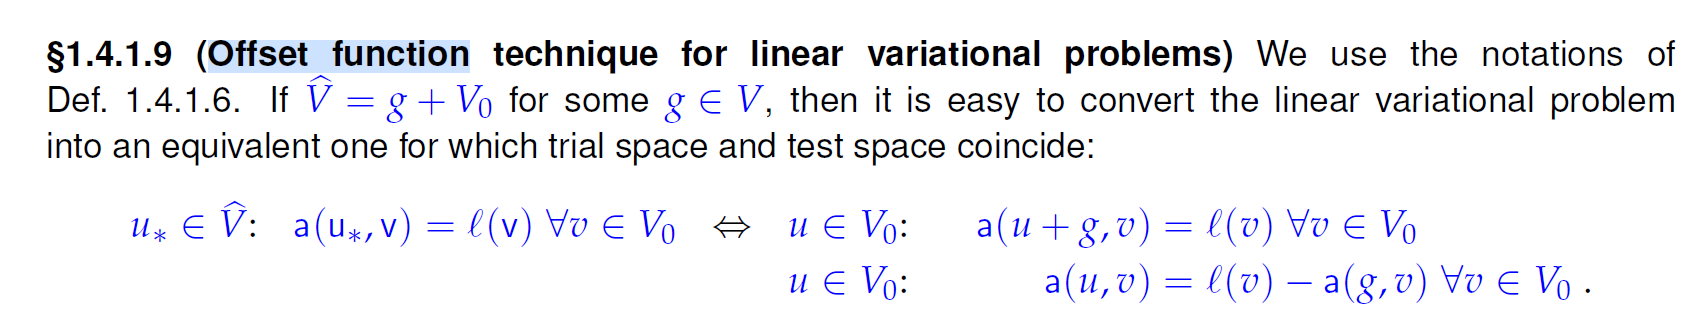
\includegraphics{week03/ex_offset_function.png}
\end{figure}

\SubSectionWith{Problem 2.1}{15min.}
On Galerkin Orthogonality.
\begin{enumerate}
    \item Prove GO: $$a(u-u_h, v_h) = 0 \forall v_h \in V_{0,h}$$
    \item Find estimate of $$J(u_h) - J(u)$$ Say why this is interesting (we try to be as close as possible to original solution wrt to energy)
    \item Draw geometry intuition of orthogonality, and intuition why this is nice (we'll come back later on this with céa's later) (closest wrt. to energy)
\end{enumerate}

\begin{figure}[h]
    \centering
    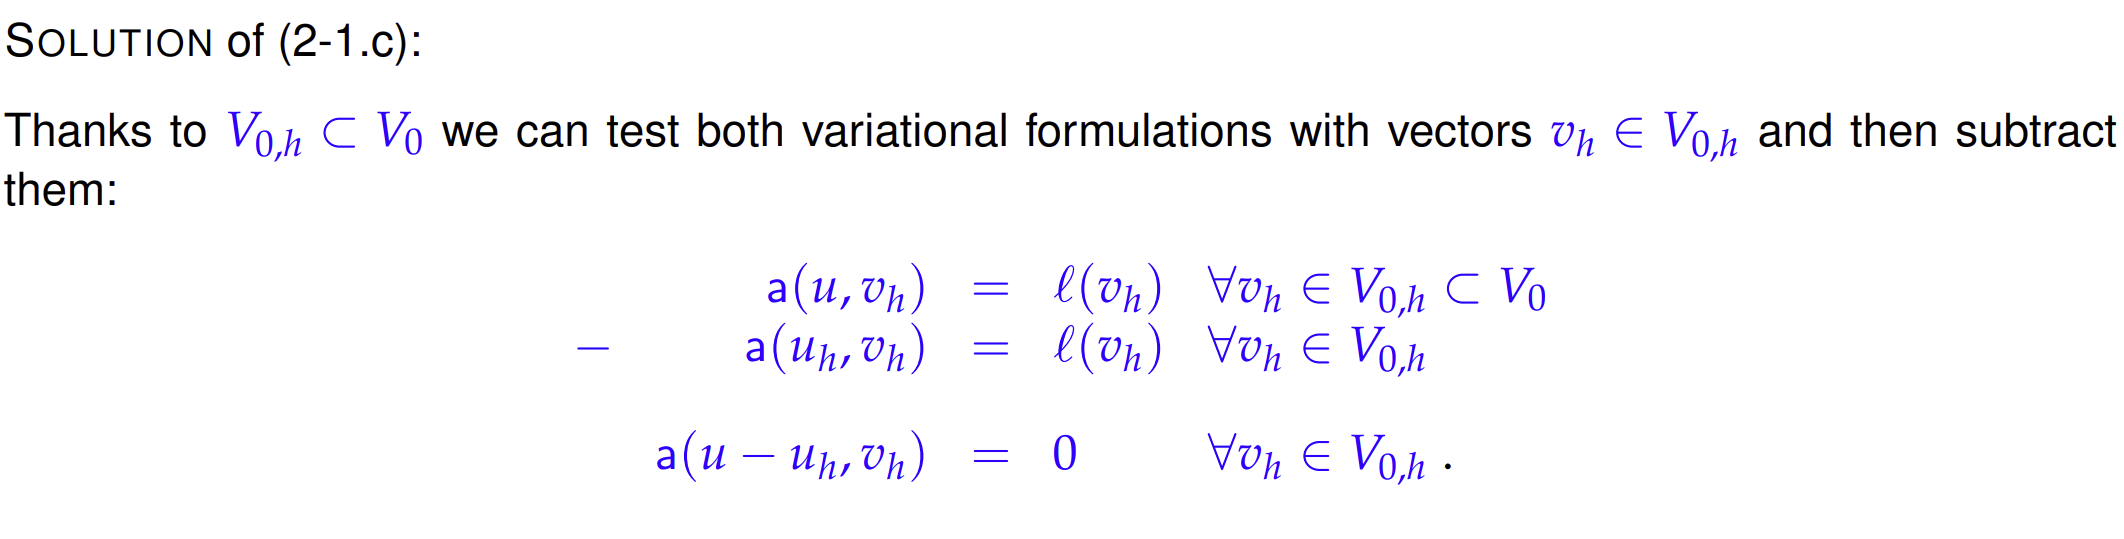
\includegraphics{week03/ex_2_1_c.png}
\end{figure}
\begin{figure}[h]
    \centering
    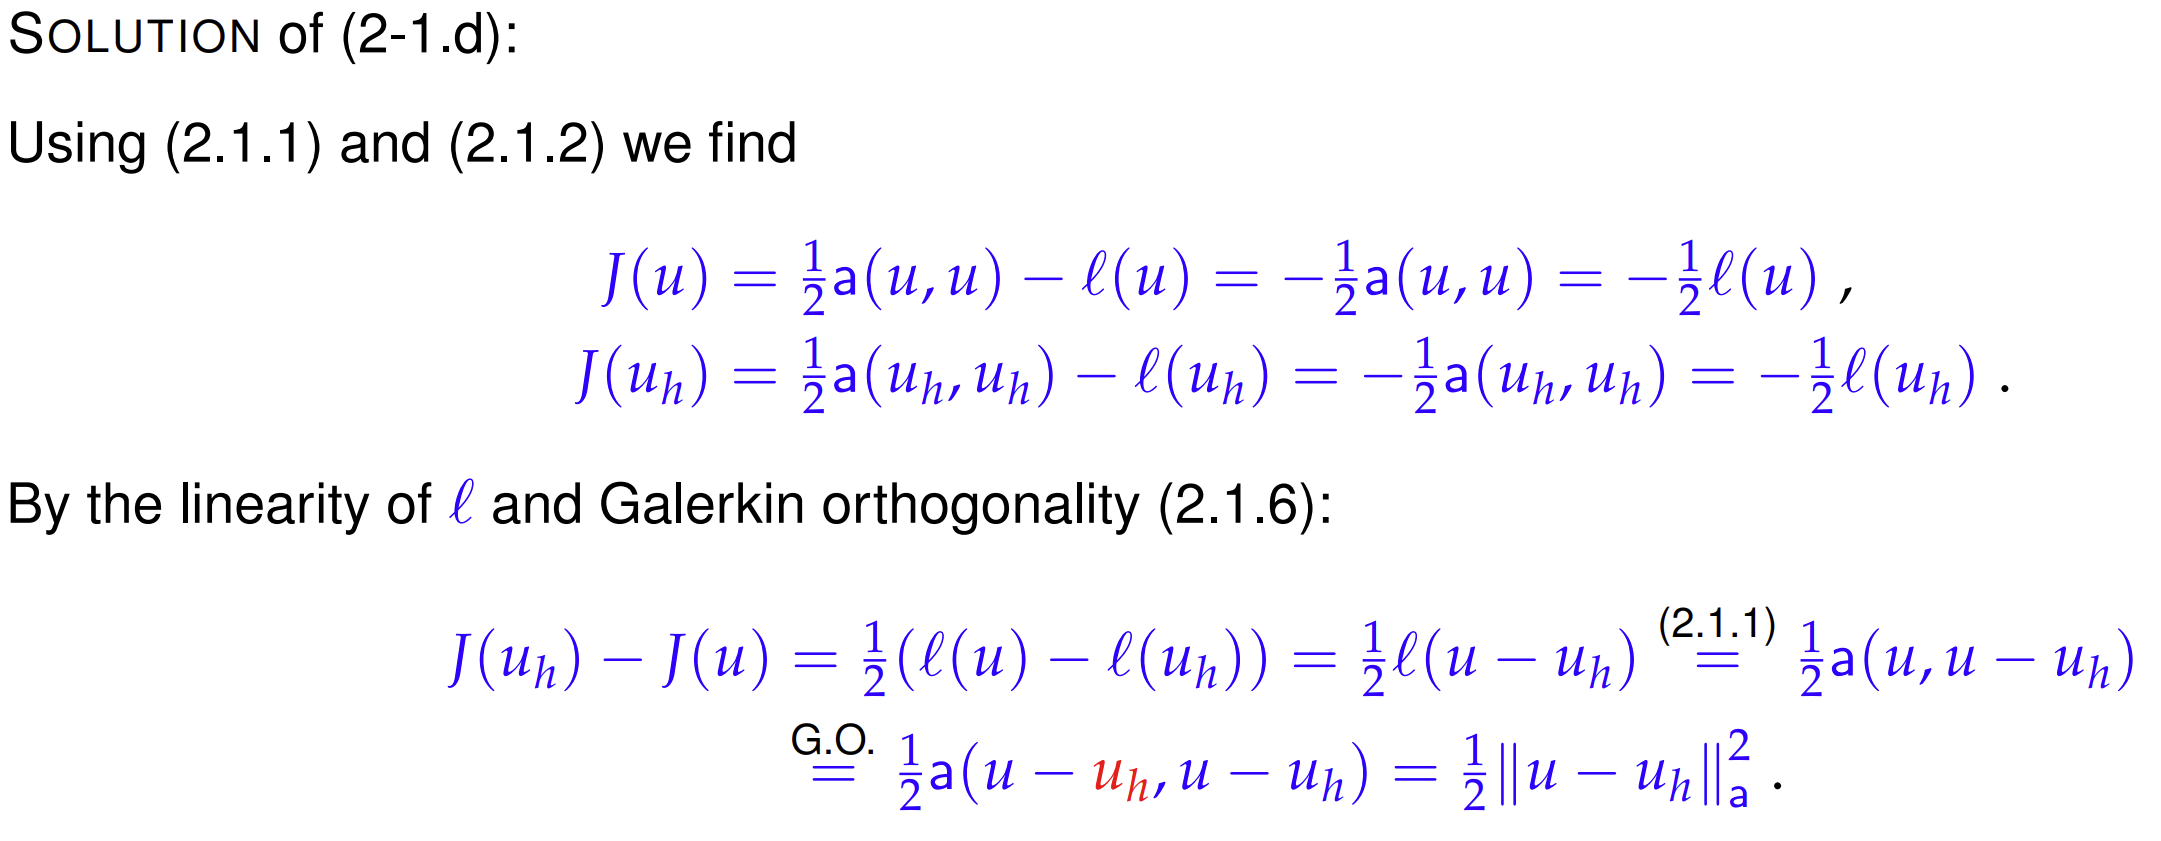
\includegraphics{week03/ex_2_1_d.png}
\end{figure}
\begin{figure}[h]
    \centering
    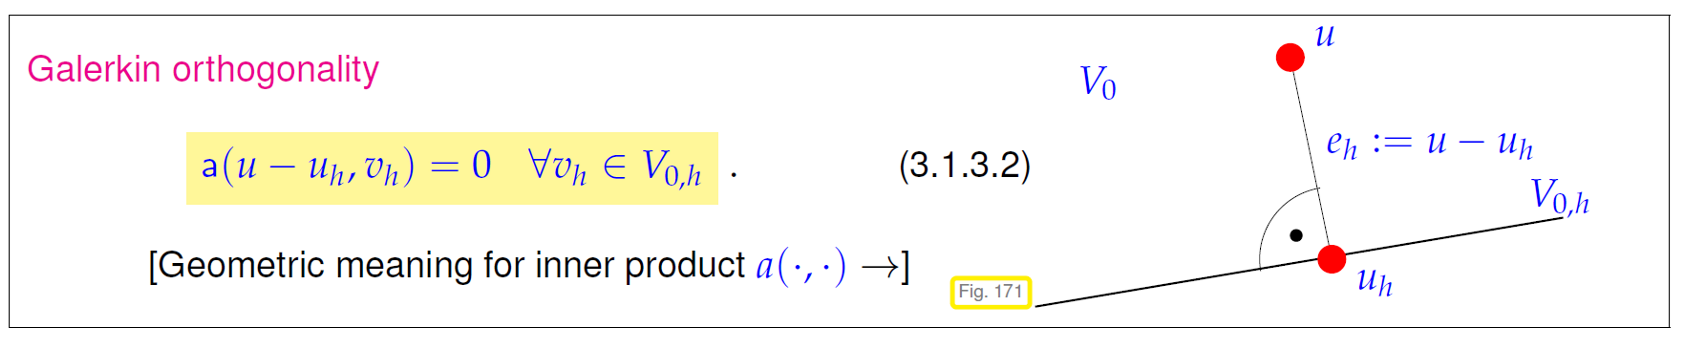
\includegraphics{week03/ex_G0.png}
\end{figure}

\SubSectionWith{Eigen Review}{15min}
(Lot of master students that didn't do CSE BSc in the class (so no NumCSE), so this is necessary)

- Sparse format, COO, CRS
- Sparse LinAlg

Then show and understand code  \url{https://github.com/erickschulz/NPDECODES/blob/master/lecturecodes/SimpleLinearFEM2D/matrix_assembler.cc}

\SubSectionWith{(If Time left) 2.2 Transformation of Galerkin Matrix}{10min.}

Main point: different basis, same solution ! Only difference is "how nice" (sparsity, condition) is the matrix.

\begin{figure}[h]
    \centering
    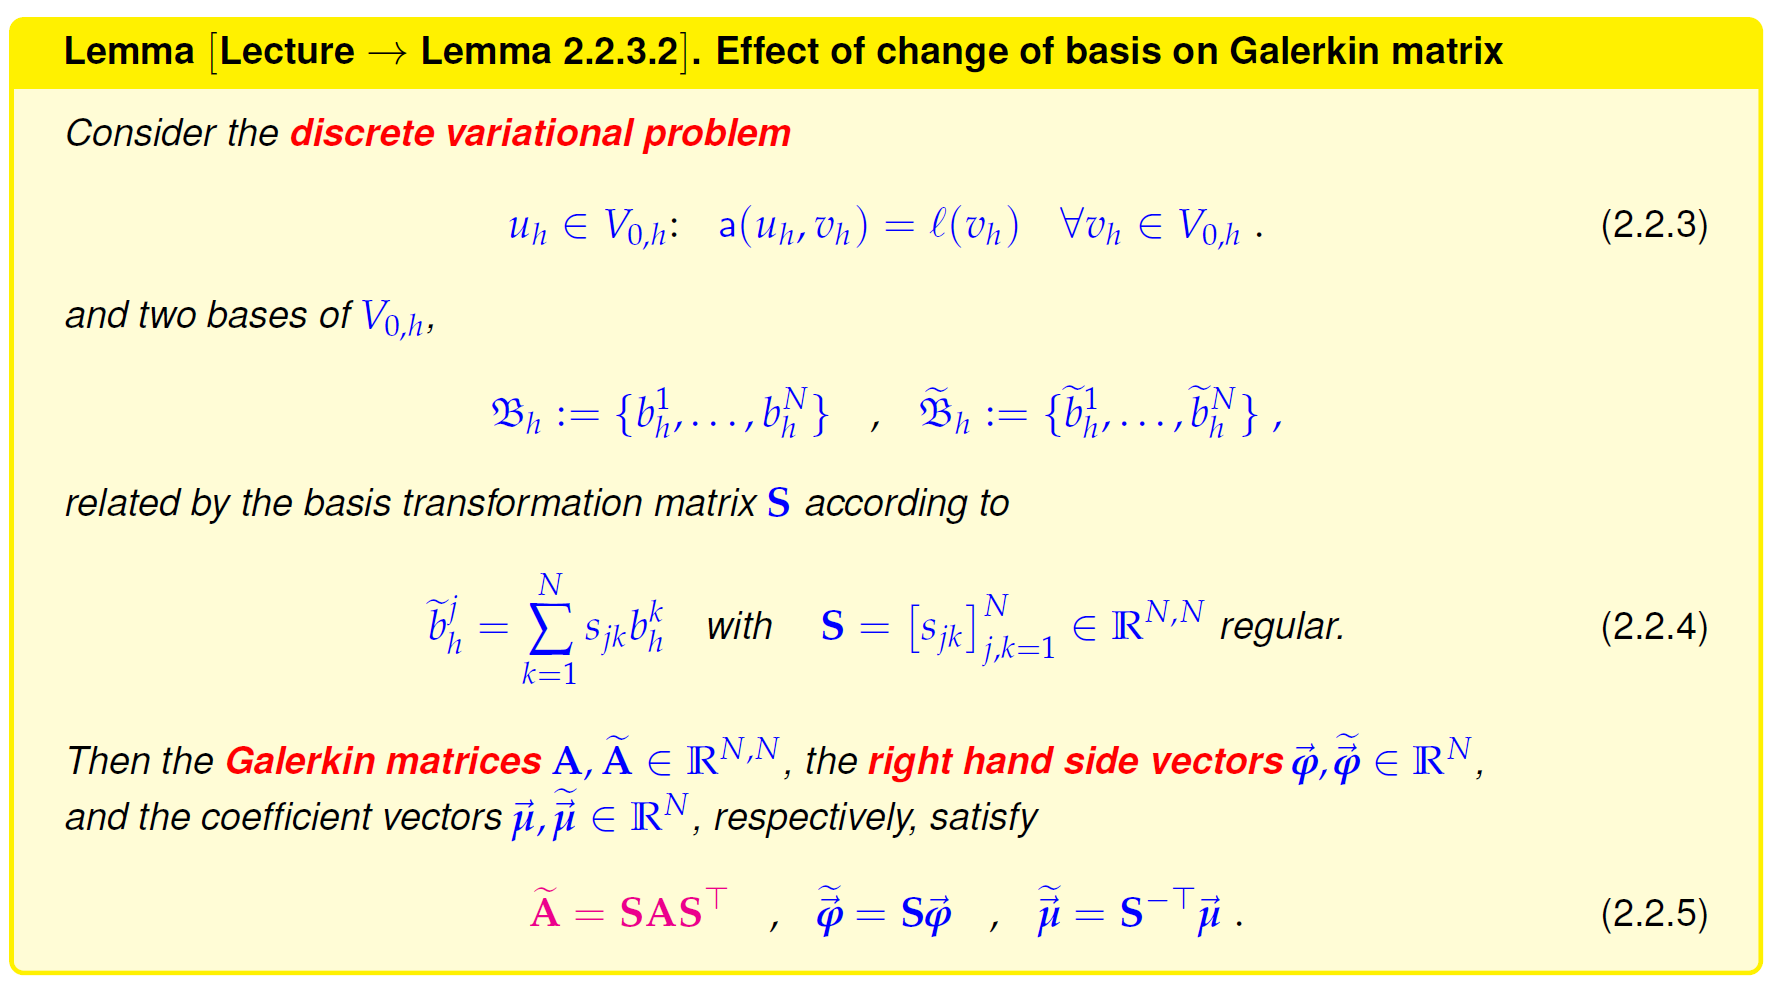
\includegraphics{week03/ex_galerkin_transformation.png}
\end{figure}


\end{document}
